
\section{System call dispatching}

\subsection{General System call layout}
The System call interface to the userspace and user processes are provided 
using the  intrinsic IPC facility provided by seL4 wherein we make the use 
of the specialized function calls \textbf{seL4\_Call}, \textbf{seL4\_Recv} and \textbf{seL4\_Send} 
to instantiate the communication between the userspace and the services
provided by our \textbf{Simple Operating System(SOS)}. \\

\subsection{IPC Protocol}
\noindent The general IPC protocol that our system maintians to initate a system call from the usersapce is to 
pass on the payload(i.e the function arguments, userspace pointers) using the Message registers/IPC buffer 
facility provided by \textbf{seL4}. And the common behavior that all system call handling code matches is to pass 
in the \textbf{SYSCALL NUMBER} in the seL4 message register(MR 0) and then the rest of the 
arguments are passed in from the message registers \textbf{1..N}. All userspace pointers are passed in as seL4Word 
pointers and are copied in the kernel using the frame iterator(talked about in the section below) in a secure way.
And the general convention followed by all the System calls is to receive back any errors in a consistent manner using the 
Message register 0 wherein \textbf{SUCCESS} represents that the users request for the particular System call has been dealt 
with consistency and the user is responded back with the results that are desired using the value reeved back from the message 
registers 1 onwards depending on the system call semantics, and \textbf{FAILURE} represents that system call has not been 
dealt with due to an error either in the system or due to the arguments passed by the user, of which the user is notified with 
correctly by passing back a desired value with regards to te system call error. All the user level library calls(libsosapi) are 
redirected back correctly into the specific user level system call(which uses the \textbf{seL4} IPC mechanism to communicate back into SOS) using the 
correct syscall number and the mapping back into the correct syscall using the number is done by the function sosapi\_init\_syscall\_table inside 
vsyscall.c. \\

\subsection{System call numbers:}
\noindent The system call number table for our Syscalls is as follows


\begin{center}
    \begin{tabular}{ |c|c|c| }
    \hline 
    \textbf{SYSCALL NUMBER} & \textbf{SYSCALL NAME} \\
    \hline
    \textbf{\_\_NR\_openat} & \textbf{sos\_sys\_open}\\ 
    \hline
    \textbf{\_\_NR\_close} &  \textbf{sos\_sys\_close}\\ 
    \hline
    \textbf{\_\_NR\_read} &  \textbf{sos\_sys\_read}\\ 
    \hline
    \textbf{\_\_NR\_write} & \textbf{sos\_sys\_write} \\
    \hline
    \textbf{SOS\_SERIAL\_CONSOLE\_OUT} & \textbf{sos\_write} \\
    \hline
    \textbf{\_\_NR\_getdents64} & \textbf{sos\_getdirent} \\
    \hline
    \textbf{\_\_NR\_fstat} & \textbf{sos\_stat} \\
    \hline
    \textbf{\_\_NR\_execve} & \textbf{sos\_process\_create} \\
    \hline
    \textbf{\_\_NR\_kill} & \textbf{sos\_process\_delete} \\
    \hline
    \textbf{\_\_NR\_getpid} & \textbf{sos\_my\_id} \\
    \hline
    \textbf{\_\_NR\_io\_getevents} & \textbf{sos\_process\_status} \\
    \hline
    \textbf{\_\_NR\_wait4} & \textbf{sos\_process\_wait} \\
    \hline
    \textbf{\_\_NR\_nanosleep} & \textbf{sos\_sys\_usleep} \\
    \hline
    \textbf{\_\_NR\_getitimer} & \textbf{sos\_sys\_time\_stamp} \\
    \hline
    \end{tabular}
\end{center} 

\subsection{SOS sycalls}
\noindent We have the following syscalls corresponding to each of the user operations that the sos thread corresponding to that user needs to handle: \\


\noindent \textbf{void sos\_serial\_console\_out(seL4\_CPtr reply, struct serial * serial, process\_data\_t * process);} \\
\noindent \textbf{void\ sos\_nanosleep(seL4\_CPtr reply);} \\
\noindent \textbf{void sos\_getitimer(seL4\_CPtr reply);} \\
\noindent \textbf{void sos\_openat(seL4\_CPtr reply, process\_data\_t * process);} \\
\noindent \textbf{void sos\_close(seL4\_CPtr reply, process\_data\_t * process);} \\
\noindent \textbf{void sos\_read(seL4\_CPtr reply, process\_data\_t * process);} \\
\noindent \textbf{void sos\_write(seL4\_CPtr reply, process\_data\_t * process);} \\
\noindent \textbf{void sos\_brk(seL4\_CPtr reply, seL4\_Word heap\_bottom, seL4\_Word * heap\_top);} \\
\noindent \textbf{void sos\_stat(seL4\_CPtr reply, process\_data\_t * process);} \\
\noindent \textbf{void sos\_getdents(seL4\_CPtr reply, process\_data\_t* process);} \\
\noindent \textbf{void sos\_getpid(seL4\_CPtr reply);} \\
\noindent \textbf{void sos\_exec(seL4\_CPtr reply, process\_data\_t * process);} \\
\noindent \textbf{void sos\_waitpid(seL4\_CPtr reply);} \\
\noindent \textbf{void sos\_process\_status(seL4\_CPtr reply, process\_data\_t * process);} \\
\noindent \textbf{void sos\_kill(seL4\_CPtr reply);} \\

\subsection{Concurrent syscall management}

\begin{figure}[h]
    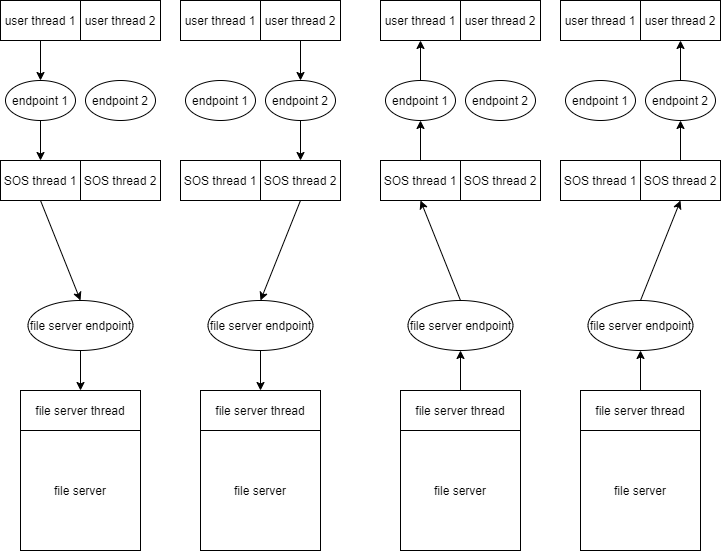
\includegraphics[width=\linewidth]{concurrent_syscalls.png}
    \caption{File server handling concurrent IO}
    \label{fig:concurrent_syscalls}
\end{figure}

\noindent The system is also capable of managing concurrent system calls as following from the execution model,
there is a kernel thread corresponding to each user thread/process and there is a separate endpoint on which 
the communication corresponding to the user thread and the sos thread is being initiated and this is what we use to 
manage the concurrent system call requests and to make sure that the system is free of any race conditions of any sort we 
add locks corresponding to any global/shared objects between each of the threads. \\
So, following off from the diagram added above whenever a user threads make in a request for any file management specific details the system call corresponding to that goes to its corresponding 
SOS thread which calls into the file server that is waiting inside the server loop on its specific endpoint, when ti receives a request it saves the reply object corresponding to that process and then goes back into the loop once again waiting for new 
requests to come by creating a new reply object specific that process and in this way we deal with the concurrent requests on the file server as all the nfs calls later as asynchronous which does'nt cause any races. 







